\documentclass[12pt]{article}
\usepackage{amsmath}
\usepackage{amsfonts}
\usepackage{mathrsfs}
\usepackage{lscape}
\usepackage{listings}
\usepackage{graphicx} % Allows for importing of figures
\usepackage{color} % Allows for fonts to be colored
\usepackage{comment} % Allows for comments to be made
\usepackage{accents} % Allows for accents to be made above and below text
%\usepackage{undertilde} % Allows for under tildes to take place for vectors and tensors
\usepackage[table]{xcolor}
\usepackage{array,ragged2e}
\usepackage{hyperref}
\usepackage{framed} % Allows boxes to encase equations and such
\usepackage{subcaption} % Allows for figures to be side-by-side
\usepackage{float} % Allows for images to not float in the document
\usepackage{booktabs}
%\usepackage[margin=0.75in]{geometry}
\usepackage[final]{pdfpages}
\usepackage{enumitem}
\usepackage[section]{placeins}

%%%%%%%%%%%%%%%%%%%%%%%%%  Function used to generate vectors and tensors %%%%%%%%%
\usepackage{stackengine}
\stackMath
\newcommand\tensor[2][1]{%
	\def\useanchorwidth{T}%
	\ifnum#1>1%
	\stackunder[0pt]{\tensor[\numexpr#1-1\relax]{#2}}{\scriptscriptstyle \sim}%
	\else%
	\stackunder[1pt]{#2}{\scriptscriptstyle \sim}%
	\fi%
}
%%%%%%%%%%%%%%%%%%%

\definecolor{mygrey}{rgb}{0.97,0.98,0.99}
\definecolor{codeblue}{rgb}{.2,0,1}
\definecolor{codered}{rgb}{1,0,0}
\definecolor{codegreen}{rgb}{0.3,0.33,0.12}
\definecolor{codegray}{rgb}{0.5,0.5,0.5}
\definecolor{codepurple}{rgb}{0.55,0.0,0.55}
\definecolor{codecyan}{rgb}{0.0,.4,.4}

\lstdefinestyle{mystyle}{
	backgroundcolor=\color{mygrey},   
	commentstyle=\color{codegreen},
	keywordstyle=\color{codeblue},
	stringstyle=\color{codepurple},
	numberstyle=\tiny\color{codegray},
	basicstyle=\footnotesize,
	breakatwhitespace=false,         
	breaklines=true,                 
	captionpos=b,                    
	keepspaces=true, 
	numbers=left,                    
	numbersep=5pt,                  
	showspaces=false,                
	showstringspaces=false,
	showtabs=false,                  
	tabsize=2
}
\lstset{style=mystyle}

\lstset{language=Matlab,backgroundcolor=\color{mygrey}}
\usepackage{lastpage}
\usepackage{fancyhdr}
\pagestyle{fancy}
%\lhead{\large{Nik Benko, John Callaway, Nick Dorsett, Martin Raming}} 
%\chead{\large{\textbf{ME EN 6960: Lab 1}}}
%\rhead{\today}
\cfoot{[\thepage\ of \pageref{LastPage}]}
\fancyheadoffset{.5cm}
\setlength{\parindent}{0cm}
\usepackage[left=.5in, right=0.50in, top=1.00in,bottom=1.00in]{geometry}
\usepackage{microtype} 
\usepackage{setspace}
\doublespace
%%%%%%%%%%%%%%%%%%%%%%%%%%%%%%%%%%%%%%%%%%%%%%%%%%%%%%%%%%%%%%%%%%%%%%%%%%


\begin{document}
\title{ Analysis of Stress Intensity Factors for Mode I and Mixed Mode with Digital Image Correlation \\ \normalsize{ME EN 6960}}
\author{Nik Benko, John Callaway, Nick Dorsett, Martin Raming}
\maketitle


\begin{abstract} 

\end{abstract}

\section{Introduction} %Nick


\section{Methods}

\subsection{Experimental Techniques} 

\subsubsection{Digital Image Correlation} % Martin
DIC is a commonly used optical technique in experimental mechanics to accurately measure full-field displacements, and rotations by capturing a sequence of images of a the surface in question. Using two cameras these measurements can be taken in 3D. If only 2D measurements are needed, as in this experiment, only one camera is needed for imaging the surface.
\\
\\
An initial digital image is taken before any loading to be used as the reference image. Here it is assumed that there are zero displacements, or rotations.  This reference image is then compared to a digital image taken once loading has occurred, also know as the deformed image. In many cases numerous digital images are captured during loading for comparison to create a sequence of displacements and rotations.  For correlation to take place an area of interest with in the images is selected and then divided into square sections known as subsets. Each subset is made up of the same number of pixels.  The subsets are matched in the reference and deformed images though a correlation function with in the DIC algorithm. By corresponding each pixel to an actual unit of length deformations and rotations can then be tracked using a DIC algorithm.
\\
\\
For the DIC algorithm to be effective each subset must contain enough unique features.  These features are related to contrast or pixel values.A high-contrast grainy surface is desired to create such usable features. In practice this is known as the speckle pattern. A good speckle pattern consists of a uniformly dispersed speckles of  random shapes and varying sizes. The size of the speckles needed will depend on the size of the specimen and focusing distances. For example a small specimen with the camera close will require very small speckles while a larger specimen with the camera backed off larger speckles are needed. 

\subsubsection{Experimental Determination of Displacement Fields} %John
Mode 1 displacement fields can be obtained by loading a specimen that has an edge crack in a three point configuration. This configuration and specimen geometry is given in Figure \ref{fig:Geometry}. Alignment of the roller directly above the crack tip creates pure bending around the crack, which induces only mode I crack opening, and therefore mode I displacement fields.
\\ \\
Mixed mode displacement fields can be obtained by inducing eccentricity in the previously described three point loading configuration. This can be done by moving one of the lower support rollers, creating a combination of bending (Mode I) and shear (Mode II) around the crack. This configuration is given in Figure \ref{fig:Geometry_Mixed}.  

\subsubsection{Calculation of Stress Intensity Factors} %john - still need to add references
Theoretical mode I stress intensity factors ($K_{I}$) can be calculated using the closed form equation:
\begin{equation}
K_{I} = Y\sigma\sqrt{\pi a}
\end{equation}
where $\sigma$ is the farfield stress, a is the crack length and Y is a geometric factor specific to the loading configuration and specimen geometry. Using the solution developed in \textit{The Stress Analysis of Cracks Handbook}, the stress intensity factor for the single edge notched bend specimen being examined is:
\begin{equation}
K_{I} = \frac{P}{B\sqrt{W}}\Bigg(\frac{\frac{3S}{W}\sqrt{\frac{a}{w}}}{2(1+\frac{2a}{w})(1-\frac{a}{w})^{1.5}}\Bigg)\Bigg[1.99-\frac{a}{w}\Big(1-\frac{a}{w}\Big)\Big[2.15-3.93\Big(\frac{a}{w}\Big)+2.7\Big(\frac{a}{w}\Big)^2\Big]\Bigg]
\end{equation}
where P is the applied load, W is the specimen width, B is the specimen thickness and a is the crack length. 
\\ \\
Experimental mode I stress intensity factors can be found using the experimental displacement fields. From the Westergaard solution, the displacements around the crack can be described by the following equations:
\begin{equation}
u_{x} = \frac{K_{I}}{8\mu \pi}\sqrt{2\pi r}\bigg[(2\kappa-1)cos\bigg(\frac{\theta}{2}\bigg)-cos\bigg(\frac{3\theta}{2}\bigg)\bigg]
\end{equation}
\begin{equation}
u_{y} = \frac{K_{I}}{8\mu \pi}\sqrt{2\pi r}\bigg[(2\kappa+1)sin\bigg(\frac{\theta}{2}\bigg)-sin\bigg(\frac{3\theta}{2}\bigg)\bigg]
\end{equation}
where (r,$\theta$) are the polar coordinate of the point, $\mu$ is the shear modulus and $\kappa$ is $\frac{3-\nu}{1+\nu}$ ($\nu$ is Poisson's ratio) for the plane stress state of the experiment.
\\ \\
    
\subsection{Procedure} %Martin
The experiment was conducted with a thin rectangular PMAA (acrylic) specimen .  To simulate a crack the specimen was cut with a bandsaw directly in the center to a length of ??. This  method was chosen to allow for a blunt crack tip so that premature failure of the specimen does not occur while testing.  One side of the plate was painted  completely white and then speckled using a black aerosol paint.  The black paint was applied in a way that allowed for random speckling with in a size range that would allow for proper DIC measurements.
\\ \\
To extract mode I data the  specimen was placed in a three-point bend fixture with in an electronic screw-driven Instron machine as figure ? shows. A light load of about 7N was used to hold the specimen in place.
The DIC setup consisted of one camera with ??mm lens mounted to a tripod.  Two green lights with flexible attachments were positioned and aligned to provide adequate lighting. With the DIC system in place the aperture to the camera was opened fully and the camera lens was then focused referencing the area around the crack tip. Next the aperture and light control were adjusted so that focus was maintained with no over exposure. 
\\
\\
We then took several images to obtain an initial reference and to get an estimate of unwanted noise. From here we incremented the load on the specimen while subsequently taking an image at each increment. Care was taken to record the load as close to the point in time that the image was captured since the specimen would relax with in the fixture resulting in a steady decreasing load. Once the threshold of 300N was reached we unloaded the specimen.  For mixed mode load we adjusted the three-point fixture to create asymmetric loading. This was achieved by simply moving one support towards the center.  This lead to a gap of four inches from one support to the center on one side and two inches on the other. Just as before the camera was focused and adjusted fallowing incremental loading with correlated images. Table ?? shows the sequence for each load and the correlated image number for both mode I and mode II.  

\subsection{Error and Uncertainties} %Martin

\section{Results}%Nik

\section{Discussion}%Nik

\section{Conclusion}%Nick

\section{Figures}
% DIC setup
\begin{figure}[H]
	\centering
	\includegraphics[width=1\textwidth]{DIC Setup.png}
	\caption{The specimen is mounted to the fixture with the DIC system in place, here the camera is fixed to a tripod and two adjustable lights are seen on either side.}
	\label{fig:DIC}
\end{figure}

% Mode I Specimen geometry
\begin{figure}[H]
	\centering
	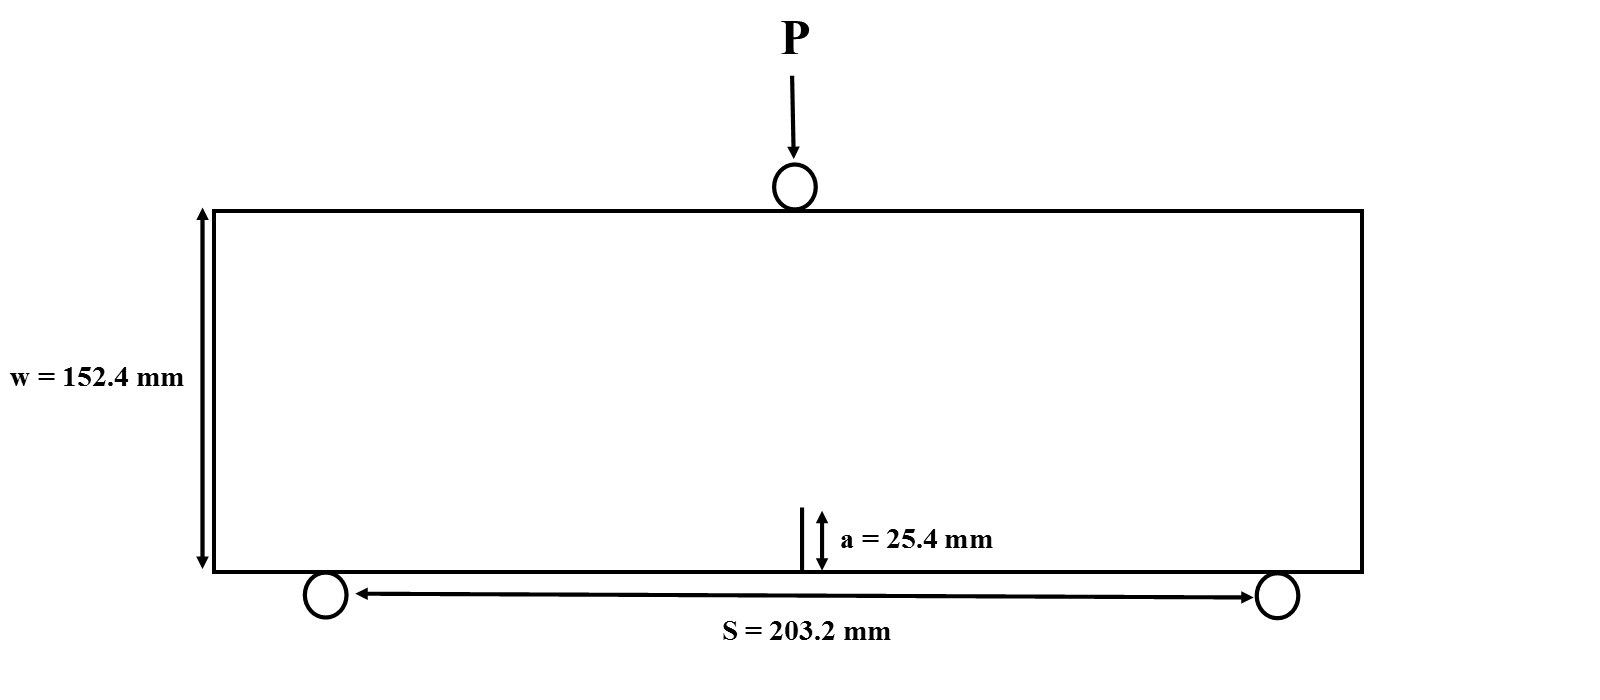
\includegraphics[width=1\textwidth]{Geometry.png}
	\caption{Three point loading configuration of specimen, where S = 0.2032 m, w = 0.1524 m, a = 0.0254 m and a specimen thickness (B) of 0.00875 m. Applied load, P, is applied to the top roller}
	\label{fig:Geometry}
\end{figure}

% Mixed Mode Specimen Geometry
\begin{figure}[H]
	\centering
	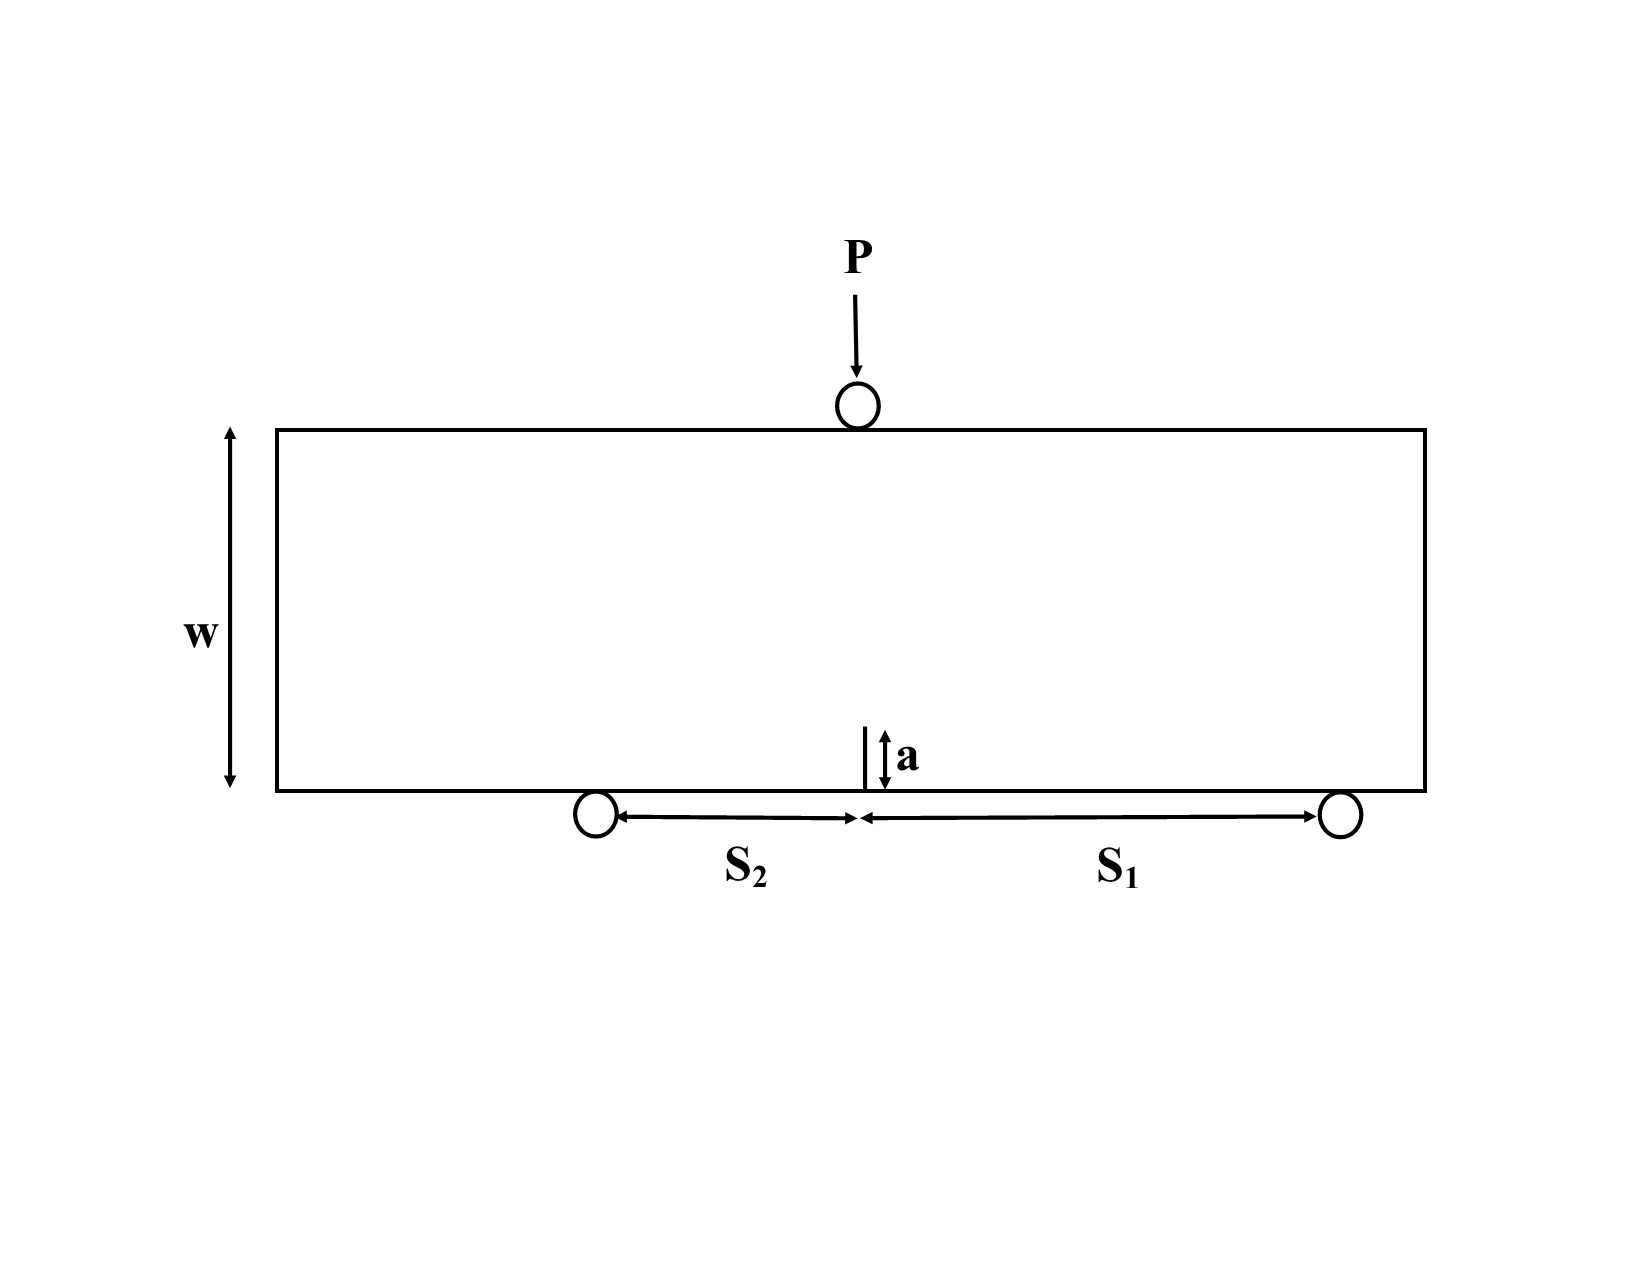
\includegraphics[width=1\textwidth]{Geometry_Mixed.png}
	\caption{Three point loading configuration of specimen, where $S_{1}$ = 0.1016 m, $S_{2}$ = 0.0508 m, w = 0.1524 m, a = 0.0254 m, and a specimen thickness (B) of 0.00875 m. Applied load, P, is applied to the top roller}
	\label{fig:Geometry_Mixed}
\end{figure}	 
\section{Tables}
%Material Properties:
%\begin{table}[h]\footnotesize
%	\centering
%	\begin{tabular}{ |l|l|l|l|l|l| }
%		\hline
%		Parameter&$\mathbf{E_1}$& $\mathbf{E_2}$ & $\mathbf{G_{12}}$ & $\mathbf{\nu_{12}}$ & $\mathbf{\nu_{21}}$ \\ \hline
%		Value& 114 GPa & 8.3 GPa& 3.93 GPa &0.33 & 0.02\\ \hline
%	\end{tabular}
%	\caption{T800-3900 Material Properties}
%	\label{tab:Material Properties}%
%\end{table}
% All layups
\
\section{Appendix}

\subsection{equations}


\subsection{Code}

\begin{verbatim}

\end{verbatim}


\bibliographystyle{IEEEtran}
\bibliography{Lab1Bib}
\end{document}